\documentclass{divers}

\renewcommand{\destinataire}{Joueurs}
\renewcommand{\numberdoc}{0}
\newcommand\twodigits[1]{%
  \ifnum#1<10 0#1\else #1\fi
}
\newcommand{\tablenum}[5]{
  \begin{tikzpicture}
    \newcommand{\scale}{#1}
    \newcommand{\ncol}{#2}
    \newcommand{\startpos}{#3}
    \newcommand{\last}{#4}
    \newcommand{\labelnum}{#5}
    \foreach \i in {1,...,\last}
    {
      \pgfmathtruncatemacro{\y}{(\i + \startpos)/\ncol};
      \pgfmathtruncatemacro{\x}{(\i + \startpos) - \ncol*\y};
      \draw (\x/\scale, -\y/\scale) node {\twodigits{\i}};
    }
    \node (chance) at (2, 0) {\labelnum} ;
  \end{tikzpicture}
}

\usepackage{tasks}
\settasks{label=\textbf{\alph*.}, label-format=\bfseries, label-offset=1em, label-align=right, before-skip =\smallskipamount, after-item-skip=0pt}

\usepackage{makecell}
\usepackage{array}

% tetrahedron

\pgfdeclareshape{fourside}{

\anchor{center}{\pgfpointorigin} % within the node, (0,0) is the center
\anchor{text}    % this is used to center the text in the node
    {\pgfpoint{-.5\wd\pgfnodeparttextbox}{-.5\ht\pgfnodeparttextbox}}

\foregroundpath{ % draw border
 \pgfpathmoveto{\pgfpoint{0cm}{.3cm}}
 \pgfpathlineto{\pgfpoint{.433cm}{-.45cm}}
 \pgfpathlineto{\pgfpoint{-.433cm}{-.45cm}}
 \pgfpathlineto{\pgfpoint{0cm}{.3cm}}
 \pgfusepath{draw}  %draw border
 \pgfusepath{draw}  %draw rectangle
}}

% cubic

\pgfdeclareshape{sixside}{
\anchor{center}{\pgfpointorigin}    % within the node, (0,0) is the center

\anchor{text}   % this is used to center the text in the node
    {\pgfpoint{-.5\wd\pgfnodeparttextbox}{-.5\ht\pgfnodeparttextbox}}

\foregroundpath{ % draw border
 \pgfpathrectanglecorners{\pgfpoint{.4cm}{.4cm}}{\pgfpoint{-.4cm}{-.4cm}}
 \pgfusepath{draw}  %draw rectangle
}}

% octahedron

\pgfdeclareshape{eightside}{
\anchor{center}{\pgfpointorigin}    % within the node, (0,0) is the center

\anchor{text}   % this is used to center the text in the node
    {\pgfpoint{-.5\wd\pgfnodeparttextbox}{-.5\ht\pgfnodeparttextbox}}

\foregroundpath{ % draw border
 \pgfpathmoveto{\pgfpoint{0cm}{.5cm}}
 \pgfpathlineto{\pgfpoint{.433cm}{.25cm}}
 \pgfpathlineto{\pgfpoint{.433cm}{-.25cm}}
 \pgfpathlineto{\pgfpoint{0cm}{-.5cm}}
 \pgfpathlineto{\pgfpoint{-.433cm}{-.25cm}}
 \pgfpathlineto{\pgfpoint{-.433cm}{.25cm}}
 \pgfpathlineto{\pgfpoint{0cm}{.5cm}}
 \pgfpathlineto{\pgfpoint{.433cm}{-.25cm}}
 \pgfpathlineto{\pgfpoint{-.433cm}{-.25cm}}
 \pgfpathlineto{\pgfpoint{0cm}{.5cm}}
 \pgfusepath{draw}  %draw interiaor
}}

% decahedron

\pgfdeclareshape{tenside}{
\anchor{center}{\pgfpointorigin}    % within the node, (0,0) is the center

\anchor{text}   % this is used to center the text in the node
    {\pgfpoint{-.5\wd\pgfnodeparttextbox}{-.5\ht\pgfnodeparttextbox}}

\foregroundpath{ % draw border
 \pgfpathmoveto{\pgfpoint{0cm}{.5cm}}
 \pgfpathlineto{\pgfpoint{.294cm}{-.154cm}}
 \pgfpathlineto{\pgfpoint{0cm}{-.3cm}}
 \pgfpathlineto{\pgfpoint{-.294cm}{-.154cm}}
 \pgfpathlineto{\pgfpoint{0cm}{.5cm}}
 \pgfpathlineto{\pgfpoint{.475cm}{.1cm}}
 \pgfpathlineto{\pgfpoint{.475cm}{-.1cm}}
 \pgfpathlineto{\pgfpoint{0cm}{-.5cm}}
 \pgfpathlineto{\pgfpoint{-.475cm}{-.1cm}}
 \pgfpathlineto{\pgfpoint{-.475cm}{.1cm}}
 \pgfpathlineto{\pgfpoint{0cm}{.5cm}}
 \pgfpathmoveto{\pgfpoint{.294cm}{-.154cm}}
 \pgfpathlineto{\pgfpoint{.475cm}{-.1cm}}
 \pgfpathmoveto{\pgfpoint{-.475cm}{-.1cm}}
 \pgfpathlineto{\pgfpoint{-.294cm}{-.154cm}}
 \pgfpathmoveto{\pgfpoint{0cm}{-.5cm}}
 \pgfpathlineto{\pgfpoint{0cm}{-.3cm}}
 \pgfusepath{draw}  %draw interiaor
}}

% dodecahedron

\pgfdeclareshape{twelveside}{
\anchor{center}{\pgfpointorigin}    % within the node, (0,0) is the center

\anchor{text}   % this is used to center the text in the node
    {\pgfpoint{-.5\wd\pgfnodeparttextbox}{-.5\ht\pgfnodeparttextbox}}

\foregroundpath{ % draw border
 \pgfpathmoveto{\pgfpoint{0cm}{.5cm}}
 \pgfpathlineto{\pgfpoint{0.294cm}{.405cm}}
 \pgfpathlineto{\pgfpoint{.475cm}{.173cm}}
 \pgfpathlineto{\pgfpoint{.475cm}{-.173cm}}
 \pgfpathlineto{\pgfpoint{.294cm}{-.405cm}}
 \pgfpathlineto{\pgfpoint{0cm}{-.5cm}}
 \pgfpathlineto{\pgfpoint{-.294cm}{-.405cm}}
 \pgfpathlineto{\pgfpoint{-.475cm}{-.173cm}}
 \pgfpathlineto{\pgfpoint{-.475cm}{.173cm}}
 \pgfpathlineto{\pgfpoint{-.294cm}{.405cm}}
 \pgfpathlineto{\pgfpoint{0cm}{.5cm}}
 \pgfpathlineto{\pgfpoint{0cm}{.349cm}}
 \pgfpathlineto{\pgfpoint{.332cm}{.108cm}}
 \pgfpathlineto{\pgfpoint{.205cm}{-.282cm}}
 \pgfpathlineto{\pgfpoint{-.205cm}{-.282cm}}
 \pgfpathlineto{\pgfpoint{-.332cm}{.108cm}}
 \pgfpathlineto{\pgfpoint{0cm}{.349cm}}
 \pgfpathmoveto{\pgfpoint{.475cm}{.173cm}}
 \pgfpathlineto{\pgfpoint{.332cm}{.108cm}}
 \pgfpathmoveto{\pgfpoint{.294cm}{-.405cm}}
 \pgfpathlineto{\pgfpoint{.205cm}{-.282cm}}
 \pgfpathmoveto{\pgfpoint{-.294cm}{-.405cm}}
 \pgfpathlineto{\pgfpoint{-.205cm}{-.282cm}}
 \pgfpathmoveto{\pgfpoint{-.475cm}{.173cm}}
 \pgfpathlineto{\pgfpoint{-.332cm}{.108cm}}
 \pgfusepath{draw}  %draw interiaor
}}

% icosohedron

\pgfdeclareshape{twentyside}{
\anchor{center}{\pgfpointorigin} % within the node, (0,0) is the center

\anchor{text}    % this is used to center the text in the node
    {\pgfpoint{-.5\wd\pgfnodeparttextbox}{-.5\ht\pgfnodeparttextbox}}

\foregroundpath{ % draw border
 \pgfpathmoveto{\pgfpoint{0cm}{.5cm}}
 \pgfpathlineto{\pgfpoint{.454cm}{.262cm}}
 \pgfpathlineto{\pgfpoint{.454cm}{-.262cm}}
 \pgfpathlineto{\pgfpoint{0cm}{-.5cm}}
 \pgfpathlineto{\pgfpoint{-.454cm}{-.262cm}}
 \pgfpathlineto{\pgfpoint{-.454cm}{.262cm}}
 \pgfpathlineto{\pgfpoint{0cm}{.5cm}}
 \pgfpathlineto{\pgfpoint{0cm}{.292cm}}
 \pgfpathlineto{\pgfpoint{.253cm}{-.146cm}}
 \pgfpathlineto{\pgfpoint{-.253cm}{-.146cm}}
 \pgfpathlineto{\pgfpoint{0cm}{.292cm}}
 \pgfpathlineto{\pgfpoint{.454cm}{.262cm}}
 \pgfpathlineto{\pgfpoint{.253cm}{-.146cm}}
 \pgfpathlineto{\pgfpoint{0cm}{-.5cm}}
 \pgfpathlineto{\pgfpoint{-.253cm}{-.146cm}}
 \pgfpathlineto{\pgfpoint{-.454cm}{.262cm}}
 \pgfpathlineto{\pgfpoint{0cm}{.292cm}}
 \pgfpathmoveto{\pgfpoint{.454cm}{-.262cm}}
 \pgfpathlineto{\pgfpoint{.253cm}{-.146cm}}
 \pgfpathmoveto{\pgfpoint{-.454cm}{-.262cm}}
 \pgfpathlineto{\pgfpoint{-.253cm}{-.146cm}}
 \pgfusepath{draw}  %draw interiaor
}}
% macros for nodes, #1 = dice value

\def\fourside#1{node[fourside,draw=black]{#1}}
\def\sixside#1{node[sixside,draw=black]{#1}}
\def\eightside#1{node[eightside,draw=black]{#1}}
\def\tenside#1{node[tenside,draw=black]{#1}}
\def\twelveside#1{node[twelveside,draw=black]{#1}}
\def\twentyside#1{node[twentyside,draw=black]{#1}}


\title{Suivi des caractéristiques}

\begin{document}

\looped{2}{
  \noindent \makebox[\textwidth]{
    \begin{tabular}{|c|c|c|c|c|c|c|c|}
      \hline
      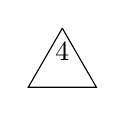
\begin{tikzpicture}[baseline=-0.5em]
        \node[fourside] (d4) at (0,0) {$4$} ;
      \end{tikzpicture} &
     \texttt{D4} et \texttt{D2 = (D4)/2} &
     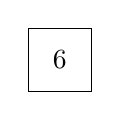
\begin{tikzpicture}[baseline=-0.5em]
     \node[sixside] (d6) at (0,0) {$6$} ;
   \end{tikzpicture} &
   \texttt{D6} et \texttt{D3 = (D6)/2} &
                                         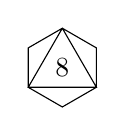
\begin{tikzpicture}[baseline=-0.5em]
                                                                                                                            \node[eightside] (d8) at (0,0) {$8$} ; 
                                                                                                                          \end{tikzpicture} &
                                                                                                                                              \texttt{D8} &
                                                                                                                                                            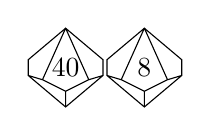
\begin{tikzpicture}[baseline=-0.5em]
                                                                                                                                                              \node[tenside] (d10) at (0,0) {$40$} ;
                                                                                                                                                              \node[tenside] (d10) at (1,0) {$8$} ;
                                                                                                                                                            \end{tikzpicture} &
                                                                                                                                                                                \texttt{D10} et \texttt{D100 = D10 D10} \\
      \hline
    \end{tabular} 
  }
  \vspace{1em}

\noindent \makebox[\textwidth]{
  \begin{tabular}{|M{0.25\linewidth}|M{0.85\linewidth}|}
    \hline
    \makecell{
    \centerline{\adforn{64} \textbf{\textsc{Points de Vie}} \adforn{36}} \\[0.5em]
    \tablenum{1.5}{4}{-1}{20}{}
    }
    & \makecell{
      \centerline{\adforn{64} \textbf{\textsc{Santé mentale}} \adforn{36}} \\[0.5em]
    \tablenum{1.5}{21}{5}{99}{Folie perpétuelle}
    } \\

    \hline
    \makecell{
    \centerline{\adforn{64} \textbf{\textsc{Points de Magie}} \adforn{36}} \\[0.5em]
    \tablenum{1.5}{4}{-1}{20}{}
    }
    & \makecell{
      \centerline{\adforn{64} \textbf{\textsc{Chance}} \adforn{36}} \\[0.5em]
    \tablenum{1.5}{21}{5}{99}{Aucune chance}
    } \\
    \hline
  \end{tabular}
}

  \vspace{1em}
  \begin{itemize*}[label=$\square$, itemjoin = \hspace{1em}]
  \item Inconscient
  \item Mourant
  \item Blessé grave
  \item Folie temporaire
  \item Folie permanente
  \end{itemize*}
  \vfill
}


\end{document}